
% 
% Annual Cognitive Science Conference
% Sample LaTeX Paper -- Proceedings Format
% 

% Original : Ashwin Ram (ashwin@cc.gatech.edu)       04/01/1994
% Modified : Johanna Moore (jmoore@cs.pitt.edu)      03/17/1995
% Modified : David Noelle (noelle@ucsd.edu)          03/15/1996
% Modified : Pat Langley (langley@cs.stanford.edu)   01/26/1997
% Latex2e corrections by Ramin Charles Nakisa        01/28/1997 
% Modified : Tina Eliassi-Rad (eliassi@cs.wisc.edu)  01/31/1998
% Modified : Trisha Yannuzzi (trisha@ircs.upenn.edu) 12/28/1999 (in process)
% Modified : Mary Ellen Foster (M.E.Foster@ed.ac.uk) 12/11/2000
% Modified : Ken Forbus                              01/23/2004
% Modified : Eli M. Silk (esilk@pitt.edu)            05/24/2005
% Modified : Niels Taatgen (taatgen@cmu.edu)         10/24/2006
% Modified : David Noelle (dnoelle@ucmerced.edu)     11/19/2014

%% Change ''letterpaper'' in the following line to ''a4paper'' if you must.

\documentclass[10pt,letterpaper]{article}

\usepackage{cogsci}
\usepackage{pslatex}
\usepackage{apacite}
\usepackage{amsmath,amssymb}
\usepackage{graphicx}
\usepackage{subcaption}
\usepackage{color}
\usepackage{url}
\usepackage{todonotes}
\usepackage{mathtools}
\usepackage{stmaryrd}
\usepackage{booktabs}
\usepackage{array}
\graphicspath{{./figures/}}

%\newcommand{\url}[1]{$#1$}

\definecolor{Red}{RGB}{178,34,34}
\newcommand{\red}[1]{\textcolor{Red}{#1}}
\definecolor{Green}{RGB}{10,200,100}
\newcommand{\ndg}[1]{\textcolor{Green}{[ndg: #1]}}
\newcommand{\mf}[1]{\textcolor{Red}{[ndg: #1]}}

 \newcommand{\denote}[1]{\mbox{ $[\![ #1 ]\!]$}}


\newcommand{\subsubsubsection}[1]{{\em #1}}
\newcommand{\eref}[1]{(\ref{#1})}
\newcommand{\tableref}[1]{Table \ref{#1}}
\newcommand{\figref}[1]{Fig.~\ref{#1}}
\newcommand{\appref}[1]{Appendix \ref{#1}}
\newcommand{\sectionref}[1]{Section \ref{#1}}

\title{Graphical convention formation during visual communication}
 
\author{\begin{tabular}[htbp]{c@{\extracolsep{1em}}c@{\extracolsep{1em}}c@{\extracolsep{1em}}c} \\
{\large \bf Megumi Sano} & {\large \bf Robert X. D. Hawkins} & {\large \bf Noah D. Goodman} & {\large \bf Judith E. Fan}\\
Department of Psychology & Department of Psychology & Department of Psychology & Department of Psychology \\ 
Stanford University & Stanford University & Stanford University & Stanford University \\
\texttt{megsano@stanford.edu} & \texttt{rxdh@stanford.edu} & \texttt{ngoodman@stanford.edu} & \texttt{jefan@stanford.edu} \\
\end{tabular}
}

\begin{document}
\maketitle

\begin{abstract}
Over time, humans have developed sophisticated graphical conventions to communicate, ranging from maps to musical notation to modern data visualization. Where do these conventions come from? A key hypothesis is that the emergence of such conventions is fundamentally driven by local patterns of usage among communicators and their functional needs. In this project, we investigated how novel graphical conventions form across extended visual communication between agents. Specifically, we used an online drawing-based reference game in which two players repeatedly communicate about visual objects. On each trial, both players were shown an array of four objects; the sketcher’s goal was to draw one of these objects, the target, so that the viewer can guess the target as quickly as possible. The game included two sets of objects: objects in one set were drawn repeatedly, while those in a control set were drawn once at the beginning and again at the end of the game. Across repetitions of the repeated objects, we find that pairs discover increasingly sparse, yet effective and internally consistent ways of depicting them. While we observe gains in visual communication efficiency for all objects, they were greater for the repeated objects, suggesting both task-level and object-level benefits of repeated communication. Moreover, different pairs discovered different solutions for efficient communication, revealing the existence of multiple equilibria in the space of graphical conventions. Taken together, our findings suggest that pairs increasingly coordinate on depictions whose meanings are determined by social context rather than their perceptual properties alone. Future experiments will examine how developing such ad hoc graphical conventions support generalization to novel visual concepts.

\textbf{Keywords:}
XX; XX; XX; XX

\end{abstract}

\section{Introduction}
%% Set up problem
XX

\section{Methods}

\subsubsection{Participants}
A total of 130 unique participants (verify), who were recruited via Amazon Mechanical Turk (AMT) and grouped into pairs, completed the experiment. They were provided a base compensation of \$1.50 for participation and earned up to \$0.03 bonus for each correct trial, inversely proportional to the amount of time taken. In this and subsequent behavioral experiments, participants provided informed consent in accordance with the Stanford IRB.
\footnote{All materials and data are available at \url{https://github.com/judithfan/graphical_conventions}.}

\subsubsection{Stimuli}
%% provide justification for why we're using sets of similar objects
%% provide justification for why we're using images of real-world objects
Because our goal was to understand the formation of \textit{ad hoc} graphical conventions, we sought to construct communicative contexts wherein people could not solely rely on pre-existing conventions to distinguish objects. 
However, it was also important to use objects that were familiar and naturalistic for some good reason.
Our approach was to define sets of perceptually similar real-world objects belonging to the same basic-level category \cite{MervisRosch81_CategorizationReview}.
To accomplish this, we utilize the collection of chair objects in the ShapeNet database \cite{chang2015shapenet}. 
This shape collection is  geometrically complex, highly diverse, and abundant in the real world. 
To identify groups of perceptually similar chairs within the collection, we first extracted high-level visual features of each of the 3,096 images using a pre-trained convolutional neural network \cite{simonyan2014very}. 
We then applied principal component analysis and $k$-means clustering to the model's top-layer feature representation of the images. 
This yielded 70 clusters containing between 2 and 80 objects each (verify). To form 2 clusters of highly visually similar objects, we manually selected 8 objects from 2 of these clusters (see Figure 1). 

% In order to identify groups of objects that are drawn similarly prior to training, we applied a clustering algorithm (affinity propagation with damping = 0.9; \cite{frey2007clustering}) to the model's top-layer feature representation of drawings from the same dataset analyzed above \cite{Eitz:2012dk}. This yielded 16 clusters containing between 3 and 20 objects each. Among clusters containing at least 8 objects, we defined 8 ``visual categories'' containing 8 objects each (Table \ref{cluster_obj_list}). Each participant was randomly assigned two of these categories, and only the 16 objects from these two categories appeared as drawing targets during their session.

%% Shapenet
%% Describe goal (groups of highly similar objects that would be hard to distinguish)

%% PCA 

%% Figure 1 around here: (A) Stimuli. (B) Task (Sketcher/Viewer interface)
\begin{figure}
\begin{subfigure}{0.23\textwidth}

\includegraphics[width=\linewidth]{fig_a.jpg}
\caption{Stimuli} \label{fig:1a}
\end{subfigure}
\hspace*{\fill} 
\begin{subfigure}{0.23\textwidth}

\includegraphics[width=\linewidth]{fig_b.jpg}
\caption{Sketcher / Viewer interface} \label{fig:1b}
\end{subfigure}
\caption{} \label{fig:1}
\end{figure}


\subsubsection{Drawing Task Procedure}
%% Trial-level event structure
Drawings were collected in the context of an online, sketching-based reference game using the framework described in \citeA{Hawkins15_RealTimeWebExperiments}. The game involved two players: a \textit{sketcher} who aims to help a \textit{viewer} pick out a target object from an array of distractor objects by representing it in a sketch. On each trial, both participants were shown the same set of four objects; however, the positions of these objects were randomized for each participant. On each trial, one of the four objects was highlighted on the sketcher's screen to designate it as the target.

%% Trial-level objective of sketcher and viewer
Sketchers drew using black ink on digital canvas (pen width = 5 pixels; 300 $\times$ 300 pixels) embedded in a web browser window using Paper.js (http://paperjs.org/). Participants drew using the mouse cursor, and were not able to delete previous strokes. Each stroke was rendered on the viewer's screen immediately upon the completion of each stroke. The sketcher was instructed to take no longer than 30 seconds to produce their drawings. The viewer was allowed to guess the identity of the drawn object by clicking one of the four objects in the array even when the sketcher had not completed the drawing. Both participants received immediate task-related feedback: the sketcher learned when and which object the viewer had clicked, and the viewer learned the true identity of the target. Otherwise, the viewer had no other means of communicating with the sketcher. Both participants earned accuracy bonus points for each correct response. If the correct response was made under the 30-second time limit, they also received a speed bonus, whose amount was inversely proportional to the time taken until the response. 

%% Two conditions: repeated and control
Each pair was randomly assigned two sets containing four objects each, a repeated set and a control set, and objects in a given set always appeared together. 
The repeated set consisted of four objects from one of the two object clusters. 
The control set consisted of either the four remaining objects from the same cluster (N=XX participants) or four randomly sampled objects from the other cluster (N=XX participants).
Including both types of control sets allowed us to evaluate the specificity of the effects of repeated communication to the repeated objects: same-cluster control objects provide a measure of changes to drawings shared by all objects within that cluster, and other-cluster control objects provide a measure of changes due to task practice drawing objects from this basic-level category.

Each session consisted of three phases: pre, repetition, and post. During the repetition phase, sketchers drew the repeated objects six times each, in an interleaved order. During the pre and post phases, sketchers drew the repeated objects and control objects one time each.

Successful communication was primarily quantified as the viewer's accuracy in identifying the target. The investment of time was measured as the length of time between the beginning of the first stroke and the completion of the final stroke in each sketch. The investment of ink was measured as the number of strokes used for each sketch. 

% The \textit{pre} phase consisted of eight trials. Four of these trials are constructed using objects from the repeated condition and the other four use objects from the control condition. The \textit{repeated} phase consists of 32 trials, each of which are constructed using objects from the repeated condition. Lastly, the \textit{post} phase uses the same design as the \textit{pre} phase, in which there are four trials of the repeated condition and four trials of the control condition. 

% We used a within-subject design where for each pair, eight objects were grouped into two sets: Four objects were assigned to the repeated condition; the other four were assigned to the control condition. Each object was presented four times within a repetition, such that each object in the set of four served as the target exactly once. The assignment of objects to the conditions was randomized across pairs. 

% how repeated communication affects how people depict objects - other objects they did not repeatedly depict 
% sampled control objects with different levels of similarity to repeated objects - allows us to evaluate both generic effects of task practice, particularly when objects were drawn from a different cluster, 

% we wanted to include control objects that shared visual properties with the repeated objects in order to assess how dependent on repetition the kinds of dynamics are -- but were distinct 
% half of our participants (n=32)... 

%% Design -- pre/repeated/post

\subsubsection{Recognition Task Procedure}

\section{Results}

%% Figure 2 around here: Behavioral Results
\begin{figure}
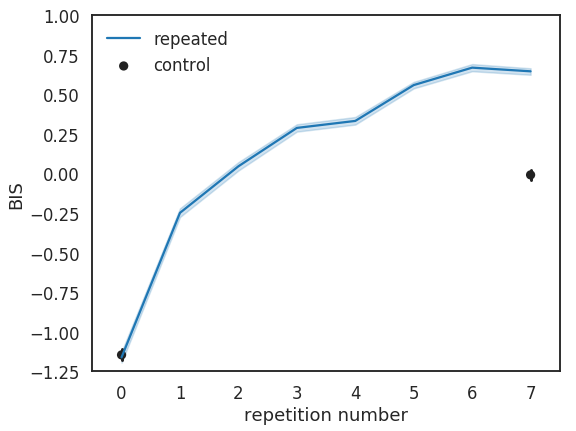
\includegraphics[width=\linewidth]{figures/fig_2.png}
\caption{Players learn to communicate more efficiently. The Balanced Integration Score (BIS) measures the difference between the $z$-scores of accuracy and drawing duration, calculated across repetitions within an interaction.} \label{fig:1a}
\end{figure}

\subsubsection{Players learn to communicate more efficiently} We predict that the repeated communication of a particular set of objects will lead to more efficient production for those objects compared to the control condition objects. To test this hypothesis, we used a composite measure called the Balanced Integration Score (BIS), which combines accuracy and a cost metric such as reaction time to measure the change in efficiency of a subject's performance at a particular task. For our experiment, we used drawing duration, the time taken from the start of the first stroke to the end of the last stroke of a sketch, as the cost metric. To calculate BIS, we normalize both accuracy and drawing duration across repetitions within subjects and take the difference between the two. We found that the efficiency of communication does increase over time (see Figure 2). 

Furthermore, while both conditions showed an increase in efficiency, we tested the extent to which improvements in efficiency from pre-test to post-test differed across the repeated and control conditions using a mixed-effects regression of condition and test phase on BIS score. Because our design was completely within-pair, we included a maximum random effect structure with random intercept, slopes, and interactions at the level of both pair and target object. We found a significant interaction: sketches of repeated targets showed a greater increase in efficiency than control targets shown only at the beginning and end ($b = 0.73. t = -2.93, p = 0.0047$; see Figure 2). We also see a similar effect when we examine number of strokes per sketch as the cost metric instead of drawing duration. This ensures that the reduction in the drawing duration and number of strokes over time is not due to the players losing interest or becoming less motivated during the game. We clearly see that while the cost of sketching decreases, the accuracy of the viewer's guess of which object the sketch is referring to increases, suggesting that this reduction is meaningful. 

% With increasing repetition number, we saw a decrease in the average number of seconds taken from the start of the first stroke to the end of the last stroke of a sketch and in the average number of strokes required to draw it. Along with this cost reduction, we saw an increase in task performance, measured by the proportion of trials for which the viewer guesses the target accurately. 




\subsubsection{XXX}

\subsubsection{Different pairs develop different conventions} To analyze how the content of the sketches change over time, we extracted the high-level perceptual features of the drawings using a pre-trained convolutional neural network. (Explain more why this is appropriate.) We define the similarity between two sketches by the correlation between their respective features.% perhaps move this similarity explanation in the earlier subsubsection. 


\subsection{Discussion}

XXXX

%\vspace{-.30cm}
\section{\bf Acknowledgments}
\small
This work was supported by ONR grant N000141310341 and a Sloan Foundation fellowship to NDG. RXDH was supported by the Stanford Graduate Fellowship and the National Science Foundation Graduate Research Fellowship under Grant No. DGE-114747.
%\vspace{-.20cm}
\bibliographystyle{apacite}

\setlength{\bibleftmargin}{.125in}
\setlength{\bibindent}{-\bibleftmargin}

\bibliography{references}


\end{document}
